\title{\color{ladrillo}\bfseries De David a la división del reino\\[4pt]\large\color{cafe}\mdseries Una casa prometida «para siempre» y un reino partido que Dios afligió «pero no para siempre»}
\author{}\date{\color{sepia}Serie «Israel, el pueblo de Dios» · Estudio 4}
\newcommand{\pt}[2]{({#1-34},{#2-31})}
\begin{document}
\maketitle\thispagestyle{empty}

\begin{abstract}\noindent
Este cuarto estudio recorre la historia de Israel desde la unción de David en Hebrón hasta la ruptura del reino bajo Roboam y Jeroboam, y muestra que la promesa de restauración atraviesa la etapa entera: Dios prometió a David una casa «para siempre» y, al dividir su reino, fijó al juicio un límite, «pero no para siempre» (1~R 11:39). La oración de Salomón prevé ya el cautiverio y el regreso del corazón (1~R 8:46--53), y los profetas y Pablo esperan un hijo de David bajo el cual Judá y Efraín vuelvan a ser un solo pueblo (Ez 37:15--28; Ro 11:26). El estudio distingue a \emph{Israel} como pueblo completo, a \emph{Israel} como reino del norte (Efraín, luego Samaria) y a \emph{Judá} como reino del sur (Judá y Benjamín, casa de David), e integra la arqueología del siglo \textsc{x} a.\,e.\,c. con sus debates y la liturgia judía.
\par\smallskip\noindent\textbf{Palabras clave:} David, Salomón, pacto davídico, templo, Sion, división del reino, Efraín, Judá, Romanos 11.
\end{abstract}

\section{Introducción}

¿Puede una promesa «para siempre» sobrevivir a un reino que se parte en dos a la tercera generación? En 2~S 7 Dios promete a David que su casa, su reino y su trono serán firmes «para siempre» (\heb{עַד־עוֹלָם}, \emph{ad olam}). Menos de un siglo después, diez tribus rechazan a su nieto con el grito «¿Qué parte tenemos nosotros con David?» (1~R 12:16). Desde entonces la Biblia habla de dos reinos, y los profetas anunciarán que volverán a ser uno bajo un rey de la casa de David (Ez 37:22, 24).

El pacto con David no sustituye la vocación de Israel como «reino de sacerdotes y nación santa» (Éx 19:6); la concentra en un rey, una ciudad y una casa de oración «para todos los pueblos» (1~R 8:41--43; Is 56:7). La división, a su vez, reproduce lo que la serie viene observando desde Abraham, un pecado que acarrea juicio y un juicio al que la propia promesa pone límite. Ahías de Silo lo formula al anunciar la ruptura: «afligiré a la descendencia de David por esto, pero no para siempre» (1~R 11:39). En esa frase, y en la oración con que Salomón dedica el templo pensando ya en un pueblo cautivo que vuelve, la restauración aparece antes de que el exilio ocurra, y desde ahí la retomarán los profetas hasta que Pablo pregunte si Dios ha desechado a su pueblo (Ro 11:1).

\begin{nota}[Tres sentidos de «Israel» desde este estudio]
En Samuel y Reyes, «Israel» puede designar al pueblo completo de las doce tribus (2~S 7:10; 1~R 8:62) o a las tribus del norte, que desde c. 931 a.\,e.\,c. forman el reino de Jeroboam, con centro en Efraín y, desde Omri, capital en Samaria (1~R 12:20; 16:24). «Judá» es la tribu y, desde la división, el reino de Judá y Benjamín con la casa de David (1~R 12:21); en 1~R 12:1, 16 y 20 «todo Israel» son solo las tribus del norte. Aquí se escribe «Israel (norte)», «reino del norte» o «Efraín» para ese segundo sentido. Las citas son traducción propia desde el hebreo (BHS) y el griego (NA28; Septuaginta según Rahlfs-Hanhart), con la numeración hebrea entre corchetes cuando difiere.
\end{nota}

\section{Marco cronológico}

La cronología descansa sobre 1~R 6:1, que sitúa el comienzo del templo en el cuarto año de Salomón, y sobre las cifras de reinado: David reinó siete años y medio en Hebrón sobre Judá y treinta y tres en Jerusalén «sobre todo Israel y Judá» (2~S 5:4--5), y Salomón cuarenta (1~R 11:42). Con la cronología de Thiele (1983), que sigue esta serie, la división cae en 931/930 a.\,e.\,c.; la escuela de Albright prefería c. 922. El primer sincronismo externo es la campaña de Sisac en el quinto año de Roboam (1~R 14:25), aunque las fechas de Sheshonq~I también se discuten (Kitchen, 1986).

\begin{center}
\begin{tikzpicture}[x=1cm,y=1cm]
\draw[line width=1.6pt,cafe,-{Latex[length=3mm]}] (0,0) -- (15.4,0);
\foreach \x/\t/\b in {0.6/{David rey de Judá en Hebrón}/{2~S 2:4; c. 1010},
                      2.6/{Rey sobre todo Israel; Jerusalén}/{2~S 5; c. 1003},
                      4.6/{El arca a Sion; pacto davídico}/{2~S 6--7},
                      6.6/{Betsabé, Absalón, Seba}/{2~S 11--20},
                      8.6/{Salomón rey}/{1~R 1--2; c. 970},
                      10.6/{Templo: 4.º año, 7 años}/{1~R 6:1, 38; c. 966--959},
                      12.6/{División del reino}/{1~R 12; c. 931/930},
                      14.6/{Sisac en Judá e Israel}/{1~R 14:25; c. 926/925}}{
  \fill[oro] (\x,0) circle (4pt);
  \node[above,font=\scriptsize\bfseries,text=ladrillo,text width=1.9cm,align=center] at (\x,0.2) {\t};
  \node[below,font=\tiny,text=sepia,text width=1.8cm,align=center] at (\x,-0.2) {\b};}
\draw[decorate,decoration={brace,amplitude=5pt,mirror},sepia] (0.4,-0.95) -- (7.0,-0.95) node[midway,below=5pt,font=\scriptsize\itshape]{David: un reino unido por pacto};
\draw[decorate,decoration={brace,amplitude=5pt,mirror},sepia] (8.4,-0.95) -- (12.8,-0.95) node[midway,below=5pt,font=\scriptsize\itshape]{Salomón: esplendor y quiebre};
\end{tikzpicture}\\[2pt]
{\footnotesize\color{sepia}\textit{Nota.} Elaboración propia. Fechas aproximadas a.\,e.\,c. según Thiele (1983); otras cronologías bajan la división a c. 922.}
\end{center}

\section{Contexto histórico y arqueológico}

Desde los años noventa, la «cronología baja» de Israel Finkelstein rebaja unos ochenta años los estratos del siglo \textsc{x}, atribuye sus obras monumentales a los omridas del norte y hace de David y Salomón jefes de un reino pequeño de las montañas de Judá (Finkelstein, 1996; Finkelstein y Silberman, 2006). Amihai Mazar (2010) defiende una «cronología convencional modificada», y Kitchen (2003) argumenta que un reino pequeño pudo crecer rápido mientras Egipto y Asiria estaban débiles.

El hallazgo más firme es la \textbf{Estela de Tel Dan} (c. 840 a.\,e.\,c.), inscripción aramea descubierta en 1993--1994 por Avraham Biran en la ciudad donde Jeroboam puso uno de sus becerros. Su autor, probablemente Hazael de Damasco, dice haber matado a [Jo]ram hijo de [Acab], «rey de Israel», y a [Ocoz]ías, rey de \heb{ביתדוד} (\emph{bytdwd}), «la casa de David» (Biran y Naveh, 1993, 1995). Es la primera mención segura de David fuera de la Biblia, y respalda desde fuera la distinción que sigue este estudio: un rey extranjero conocía dos reinos, «Israel» y la «casa de David», es decir, Judá nombrado por su dinastía. En la línea 31 de la Estela de Mesa, muy dañada, Lemaire (1994) reconstruyó también \emph{b[t]dwd}, pero Finkelstein, Na'aman y Römer (2019) propusieron leer allí un nombre propio, posiblemente Balac, y esa lectura no debe usarse como prueba firme.

\begin{center}
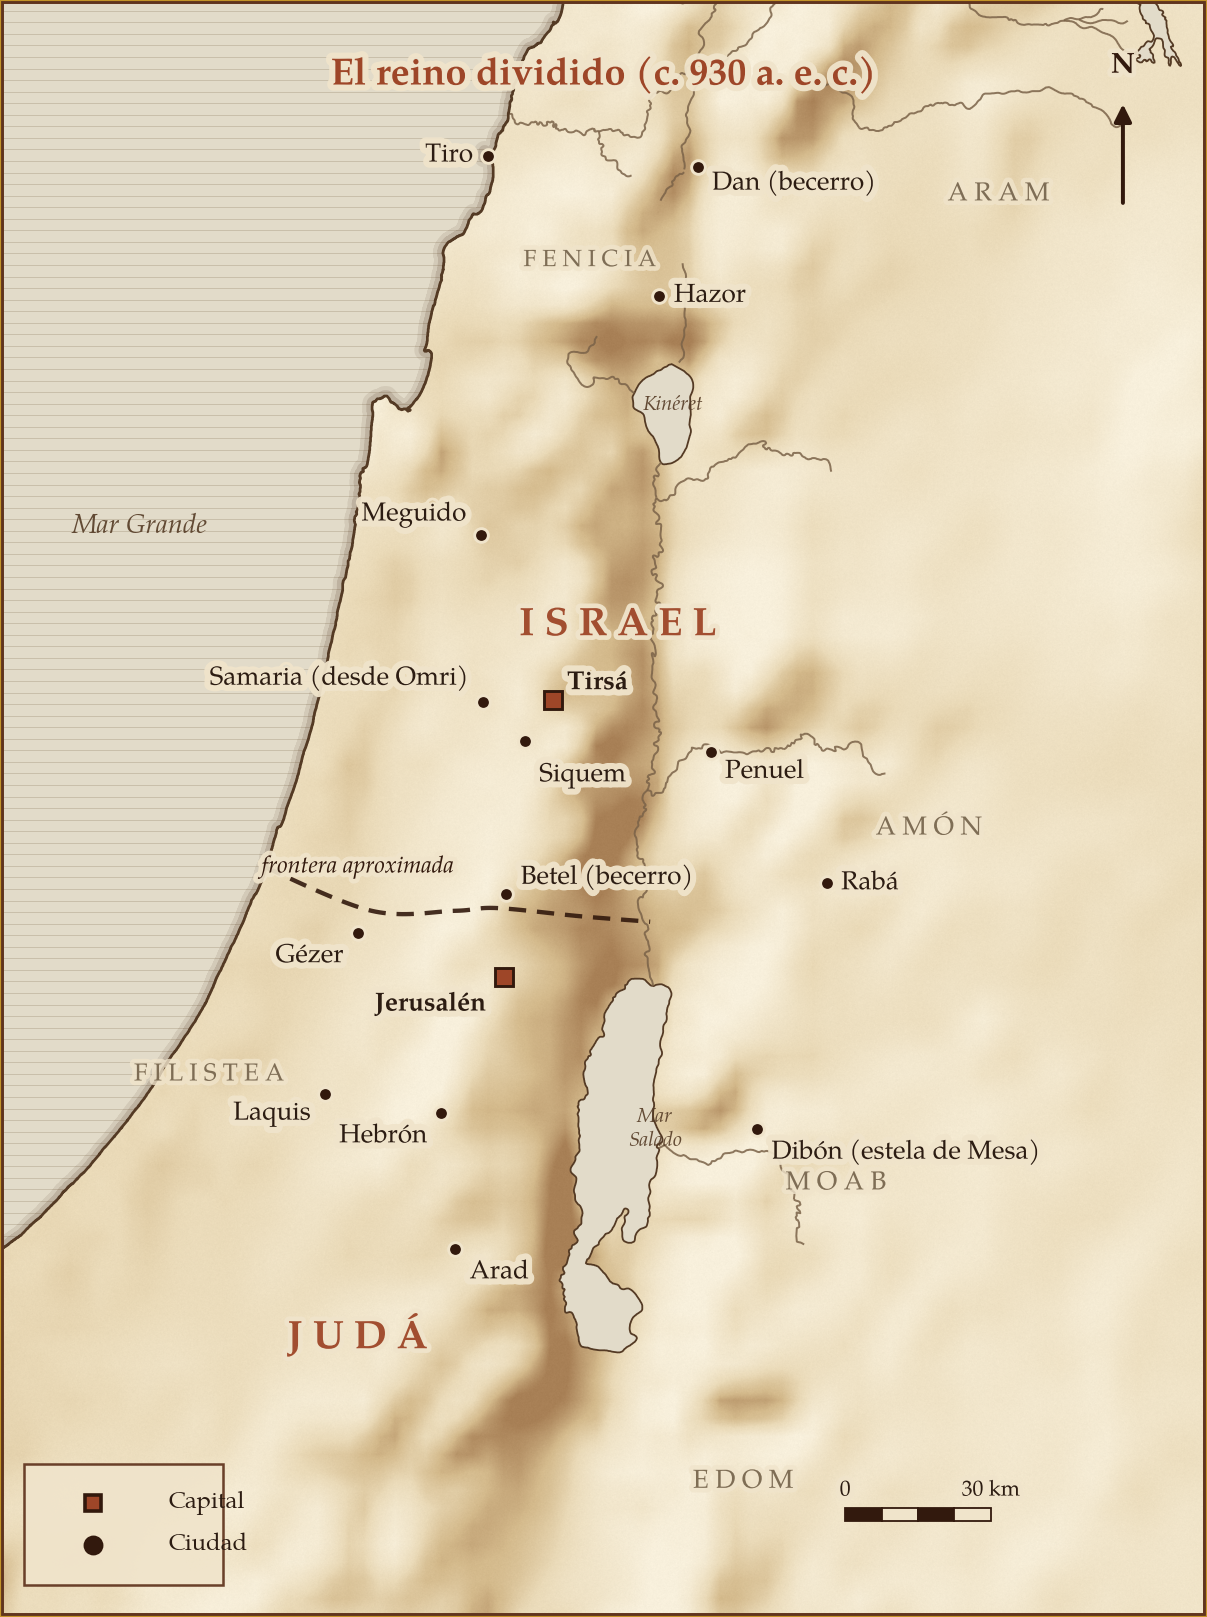
\includegraphics[width=0.36\linewidth]{mapa_division.png}\\[2pt]
\begin{minipage}{0.85\linewidth}\centering
{\footnotesize\color{sepia}\textit{Nota.} Elaboración propia: costas, lagos y ríos GSHHS/WDB y relieve sombreado (Basemap); ubicaciones antiguas aproximadas. Línea discontinua: frontera aproximada entre Israel (norte) y Judá (sur).}
\end{minipage}\end{center}

Khirbet Qeiyafa, sobre el valle de Elá, es una ciudad fortificada de c. 1020--980 a.\,e.\,c. (Garfinkel et~al., 2016) que Finkelstein y Fantalkin (2012) atribuyen a otra entidad, quizá ligada a Saúl. En Jerusalén, Eilat Mazar identificó la Gran Estructura de Piedra con el palacio de 2~S 5:11 (Mazar, 2006), y Finkelstein et~al. (2007) objetaron que los restos son de varias épocas. Del templo de Salomón no hay restos excavados, y las puertas de seis cámaras de Hazor, Meguido y Gezer, que Yadin (1958) atribuyó a Salomón a partir de 1~R 9:15, fueron fechadas por Finkelstein (1996) en el siglo \textsc{ix}; el radiocarbono no ha cerrado la cuestión. Poco después de la ruptura, Sheshonq~I grabó en Karnak una lista de unos ciento cincuenta topónimos del Levante (Kitchen, 1986). Jerusalén no figura en las partes legibles, lo que concuerda con el rescate de 1~R 14:25--26, y la lista incluye ciudades del reino del norte, cuyo rey Jeroboam había sido asilado por el propio Sisac (1~R 11:40).

\section{Desarrollo bíblico}

\subsection{Un reino unido por pacto}
Tras la muerte de Saúl, «vinieron los hombres de Judá y ungieron allí a David como rey sobre la casa de Judá» (2~S 2:4), mientras Abner proclamaba a Is-boset rey «sobre todo Israel» (2~S 2:9), un «Israel» que aquí significa las tribus del norte y de Transjordania. Siete años y medio después vinieron a Hebrón «todas las tribus de Israel» y dijeron: «Henos aquí, hueso tuyo y carne tuya somos. [\ldots] Y el rey David hizo pacto con ellos en Hebrón delante de YHWH» (2~S 5:1, 3). La adhesión de un pueblo que se reconoce emparentado se sella, con todo, con un \heb{בְּרִית} (\emph{berit}) entre el rey y los ancianos del norte (McCarter, 1984; Alter, 1999), y la tensión siguió latente: tras la rebelión de Absalón, el benjaminita Seba tocó el shofar con un grito que reaparecerá en Siquem, «No tenemos parte en David ni heredad en el hijo de Isaí. ¡Cada uno a sus tiendas, Israel!» (2~S 20:1).

David tomó «la fortaleza de Sion» (2~S 5:7), plaza jebusea en la frontera entre Judá y Benjamín, y subió a ella el arca. El Sal 78 interpreta ese traslado como una elección: Dios «desechó la tienda de José y no escogió la tribu de Efraín, sino que escogió la tribu de Judá, el monte Sion, al cual amó» (Sal 78:67--68). Sion nació así como principio de unidad y, para Efraín, como fuente de resentimiento.

\subsection{El pacto davídico: una casa para David}
En 2~S 7 se encuentra el centro de gravedad de la etapa. David quiere construir una casa para el arca, pero Natán recibe otra palabra, y el capítulo juega con \heb{בַּיִת} (\emph{báyit}), «casa», que pasa de designar el palacio (7:2) y el templo (7:5, 13) a nombrar la dinastía: «YHWH te hace saber que YHWH te hará casa» (7:11). David quería dar a Dios una casa, y es Dios quien termina dándosela a él:

\hebverso{הוּא יִבְנֶה־בַּיִת לִשְׁמִי וְכֹנַנְתִּי אֶת־כִּסֵּא מַמְלַכְתּוֹ עַד־עוֹלָם\\
אֲנִי אֶהְיֶה־לּוֹ לְאָב וְהוּא יִהְיֶה־לִּי לְבֵן}
\begin{cita}Él edificará casa a mi nombre, y yo afirmaré para siempre el trono de su reino. Yo le seré a él padre, y él me será a mí hijo. Si hace mal, yo lo castigaré con vara de hombres [\ldots]; pero mi misericordia no se apartará de él, como la aparté de Saúl. Y será firme tu casa y tu reino para siempre delante de ti, y tu trono será estable para siempre.\fuente{(2~S 7:13--16)}\end{cita}

El vocabulario de la solidez remite a quien promete. «Firme» es \heb{נֶאְמַן} (\emph{ne'emán}), de la raíz de \emph{emuná} (Gn 15:6), y «estable» y «afirmaré» proceden de \emph{kun}, «establecer»; Isaías hablará de \heb{חַסְדֵי דָוִד הַנֶּאֱמָנִים}, «las misericordias firmes de David» (Is 55:3). Lo decisivo para la restauración está en la cláusula del castigo, porque el hijo puede pecar y ser disciplinado sin que la \heb{חֶסֶד} (\emph{jésed}) se aparte de él (7:14--15). La obediencia decide si cada rey disfruta la promesa (1~R 2:4; Sal 132:12), pero no si la promesa subsiste, y por eso la Escritura la llama «pacto perpetuo» (\heb{בְּרִית עוֹלָם}, 2~S 23:5).

La casa prometida queda herida casi enseguida. Natán confronta a David por Betsabé y Urías con un «tú eres ese hombre» (\emph{atá ha-ish}, 2~S 12:7), y llegan juntos el perdón y la consecuencia: «no morirás», pero «no se apartará jamás la espada de tu casa» (12:10, 13). El Sal 51, que la tradición sitúa en este momento, pide con el verbo de Gn 1:1 un corazón limpio y «un espíritu firme» (\emph{najón}, el adjetivo del trono «estable» de 2~S 7:16); la conexión es una observación propia, pero sugiere que la estabilidad de la casa pasa por un corazón renovado, lo que Jeremías y Ezequiel anunciarán para todo el pueblo (Jer 31:33; Ez 36:26).

\subsection{Salomón y el Primer Templo}
El templo comenzó «el año cuatrocientos ochenta después que los hijos de Israel salieron de Egipto» (1~R 6:1), y la casa de YHWH aparece así como meta del Éxodo (Éx 15:17); Crónicas la sitúa en el monte Moriah, el de la Akedá (2~Cr 3:1). La dedicación se celebró en Sucot (1~R 8:2), y la nube llenó la casa como había llenado el tabernáculo (1~R 8:10--11; Éx 40:34--35). La oración de dedicación (1~R 8:22--53) enumera siete situaciones en que Israel orará hacia esa casa, y la última es el cautiverio:

\hebverso{וְהֵשִׁיבוּ אֶל־לִבָּם בָּאָרֶץ אֲשֶׁר נִשְׁבּוּ־שָׁם וְשָׁבוּ וְהִתְחַנְּנוּ אֵלֶיךָ}
\begin{cita}Si pecaren contra ti, porque no hay hombre que no peque, y los entregares delante del enemigo para que los lleven cautivos, [\ldots] y ellos volvieren en sí en la tierra adonde fueron llevados cautivos, y se convirtieren y oraren a ti [\ldots], tú oirás en los cielos [\ldots] y les harás hallar misericordia delante de los que los llevaron cautivos.\fuente{(1~R 8:46--48, 50)}\end{cita}

El hebreo entrelaza \heb{שׁוּב} (\emph{shuv}, «volver»: \emph{ve-heshivu el libbam}, \emph{ve-shavu}) con \heb{שָׁבָה} (\emph{shavá}, «llevar cautivo»: \emph{nishbu}), y el juego de sonidos dice lo que el texto enseña: al cautiverio lo vence un regreso del corazón que precede al regreso a la tierra, como en Dt 30:1--5. En la fiesta de su máxima gloria, Israel ora ya por su exilio y su vuelta, y funda la súplica en el Éxodo: «ellos son tu pueblo y tu heredad, que tú sacaste de Egipto» (8:51).

\subsection{Las causas de la división}
Salomón multiplicó caballos, mujeres y oro, lo que Dt 17:16--17 prohibía al rey. «Sus mujeres desviaron su corazón tras dioses ajenos» (1~R 11:4), y el juicio se anuncia ya acotado: «Romperé de ti el reino [\ldots]; sin embargo, no lo haré en tus días, por amor a David tu padre; daré una tribu a tu hijo por amor a David mi siervo, y por amor a Jerusalén» (11:11--13). A la idolatría se sumó la opresión. Salomón impuso \heb{מַס} (\emph{mas}), leva de trabajo forzado, «a todo Israel» (1~R 5:13 [5:27]), la palabra de Éx 1:11 para los tributos de Egipto: el rey trató a su propio pueblo como lo había hecho el faraón. Jeroboam, efraimita, dirigía la leva de «la casa de José» (1~R 11:28), y a él salió Ahías, de Silo, el antiguo santuario de Efraín, y rasgó su manto nuevo en doce pedazos: «Toma para ti diez pedazos, porque así dijo YHWH Dios de Israel: He aquí que yo rompo el reino de la mano de Salomón, y a ti te daré diez tribus [\ldots]. Y a su hijo daré una tribu, para que mi siervo David tenga lámpara todos los días delante de mí en Jerusalén» (1~R 11:31, 36). Diez más una no suman doce; 1~R 12:21 llama al reino del sur «la casa de Judá y la tribu de Benjamín», la tribu a la que dirá pertenecer Pablo (Ro 11:1). El oráculo se cierra fijando el alcance del juicio:

\begin{cita}Y yo afligiré a la descendencia de David a causa de esto, pero no para siempre.\fuente{(1~R 11:39)}\end{cita}

La última frase, \heb{אַךְ לֹא כָל־הַיָּמִים} (\emph{aj lo jol ha-yamim}), dice literalmente «pero no todos los días». La división es un juicio con plazo, y la «lámpara» (\heb{נִיר}, \emph{nir}, 11:36; 2~R 8:19), continuidad mínima de la dinastía, mantiene encendida la promesa mientras haya un hijo de David en Jerusalén (cf. Sal 132:17).

El desenlace llega en Siquem, donde Josué había renovado el pacto y adonde «todo Israel», aquí las tribus del norte, había venido para hacer rey a Roboam (1~R 12:1). Los ancianos pidieron aliviar el yugo, y Roboam prometió castigarlos «con escorpiones» (12:14). El norte retoma entonces el grito de Seba y le añade una línea: «¡Israel, a tus tiendas! ¡Provee ahora en tu casa, David!» (12:16). La palabra de 2~S 7 vuelve como fórmula de rechazo. Jeroboam es rey «sobre todo Israel», esto es, sobre el norte, y solo Judá sigue a David (12:20); cuando Roboam reúne a Judá y Benjamín para la guerra, Semaías lo detiene: «No peleéis contra vuestros hermanos, los hijos de Israel» (12:24). Consumada la ruptura, siguen siendo hermanos.

Para retener al norte, Jeroboam hizo dos becerros de oro: «He aquí tus dioses, oh Israel, los cuales te hicieron subir de la tierra de Egipto» (12:28). La frase calca la de Aarón en el Sinaí (Éx 32:4), y el reino del norte nace reproduciendo el primer pecado del pueblo redimido. Los puso en Betel y en Dan, con sacerdotes «que no eran de los hijos de Leví» (12:29--31), y aunque muchos especialistas ven en ellos pedestales del Dios invisible (Cogan, 2001), el narrador hace del «pecado de Jeroboam hijo de Nabat, que hizo pecar a Israel» el estribillo con que juzga a cada rey del norte (1~R 15:30). Según 2~Cr 11:13--17, sacerdotes, levitas y «los de todas las tribus de Israel que habían puesto su corazón en buscar a YHWH» se pasaron entonces a Judá, de modo que el reino del sur acogió también a israelitas del norte, dato que el Estudio~5 retomará.

\section{Israel como nación santa y reino de sacerdotes}

En esta etapa el llamado de Éx 19:6 adquiere rostro concreto. David sube el arca ceñido con un efod de lino, ofrece sacrificios y bendice al pueblo (2~S 6:14--18). Salomón ora por el extranjero (\emph{nojrí}) que venga por causa del nombre de Dios, «a fin de que todos los pueblos de la tierra conozcan tu nombre» (1~R 8:41--43), y el Sal 72 termina con un eco de Gn 12:3: «benditas serán en él todas las naciones» (Sal 72:17). La bendición prometida a Abraham converge en el hijo de David. La vocación se quebró en el mismo reinado, cuando el rey se hizo faraón con la leva y, después de orar por las naciones, edificó altares a sus dioses frente a Jerusalén (1~R 11:7), y cuando Jeroboam separó en el norte el sacerdocio de la elección divina. Se preservó, sin embargo, bajo la palabra de los profetas, en la confesión del rey (2~S 12:13) y en un remanente fiel que persistió en ambos reinos. Pocas décadas después, en el reino del norte, Dios se reserva siete mil que no doblaron la rodilla ante Baal (1~R 19:18), el texto que Pablo citará para afirmar que «ha quedado un remanente escogido por gracia» (Ro 11:4--5).

\section{Aporte de la tradición judía}

La tradición judía hizo de David el modelo del rey, del penitente y del Mesías esperado, y de Jerusalén el centro de la oración. En el rito babilonio de la Amidá, la bendición 14 pide la reconstrucción de Jerusalén y añade «y el trono de David establece pronto en medio de ella», y la 15 ruega: «Haz brotar pronto el renuevo de David tu siervo, y exalta su poder con tu salvación» (Sacks, 2009). El lenguaje viene de Jer 23:5 (\emph{tsémaj}, «renuevo») y del Sal 132:17, y la petición une, como los profetas, la restauración de Jerusalén y la del trono davídico. En Sucot se pide que el Misericordioso levante «la cabaña caída de David» (Am 9:11), y la costumbre de orar hacia Jerusalén, que Berajot 30a ordena en círculos concéntricos hasta el santísimo, se apoya en la oración de Salomón (1~R 8:44, 48).

Los rabinos leyeron también el pecado y el cisma. La caída de David sucedió «para enseñar el arrepentimiento al individuo» (Avodá Zará 4b--5a), mientras que de Jeroboam Sanedrín 102a narra que Dios le ofreció pasear en el Edén con él y con el hijo de Isaí si se arrepentía; cuando supo que el hijo de Isaí iría delante, respondió: «Si es así, no quiero». En el cisma veían un orgullo incapaz de aceptar el lugar de la casa de David. Antes del Nuevo Testamento, el \emph{Florilegio} de Qumrán (4Q174) aplicaba ya 2~S 7:11--14 al «Renuevo de David» de los últimos días (Vermes, 2004).

\section{La promesa de restauración}

Los textos de esta etapa ponen límite al juicio antes de que el juicio llegue, y los profetas los convertirán en esperanza de reunificación.

\begin{center}\small
\renewcommand{\arraystretch}{1.25}
\begin{tabular}{>{\RaggedRight\arraybackslash}p{2.5cm}>{\RaggedRight\arraybackslash}p{5.5cm}>{\RaggedRight\arraybackslash}p{5.9cm}}
\toprule
\textbf{Texto} & \textbf{Promesa} & \textbf{Proyección}\\
\midrule
2~S 7:14--16 & Disciplina, pero la \emph{jésed} no se aparta; casa y trono «para siempre» & Sal 89:30--37 [89:31--38]; Is 55:3; Lc 1:32--33\\
Sal 132:11, 17 & Juramento a David; renuevo y lámpara para el ungido & Jer 23:5; 33:15; Hch 2:30\\
1~R 8:46--53 & Si vuelven de corazón en el cautiverio, Dios los volverá & Dt 30:1--5; Jer 29:12--14; Dn 9:4--19\\
1~R 11:36, 39 & Una lámpara en Jerusalén; afligir «pero no para siempre» & Am 9:11; Os 3:5; Ez 37:22--25; Ro 11:1--2\\
\bottomrule
\end{tabular}\end{center}

Cuando los hechos parecían desmentirla, el Sal 89 llevó la tensión a Dios: «Señor, ¿dónde están tus antiguas misericordias, que juraste a David?» (89:49 [89:50]). Isaías responde mirando un árbol cortado. «Saldrá una vara del tronco de Isaí, y un vástago retoñará de sus raíces» (Is 11:1): queda un \heb{גֵּזַע} (\emph{guéza}), un tocón, y el profeta nombra a Isaí como si la dinastía tuviera que empezar de nuevo. Ese renuevo será «pendón a los pueblos» (11:10), y el mismo capítulo lo une a la reunión de los dos reinos:

\hebverso{אֶפְרַיִם לֹא־יְקַנֵּא אֶת־יְהוּדָה וִיהוּדָה לֹא־יָצֹר אֶת־אֶפְרָיִם}
\begin{cita}Juntará los desterrados de Israel, y reunirá los esparcidos de Judá de los cuatro confines de la tierra. [\ldots] Efraín no tendrá envidia de Judá, ni Judá afligirá a Efraín.\fuente{(Is 11:12--13)}\end{cita}

«Los desterrados de Israel» son el norte, ya deportado en tiempos de Isaías, y «los esparcidos de Judá», el sur; la envidia que separaba a los reinos desde los días de Seba ha de desaparecer, y en ello está la respuesta profética a 1~R 12. Jeremías anuncia un «renuevo justo»: «En sus días será salvo Judá, e Israel habitará confiado» (Jer 23:5--6), una salvación que alcanza a los dos reinos.

Ezequiel lleva la reunificación a un gesto. Toma dos palos, uno «para Judá» y otro «para José, palo de Efraín», y los junta en su mano (Ez 37:16--17):

\hebverso{וְעָשִׂיתִי אֹתָם לְגוֹי אֶחָד בָּאָרֶץ בְּהָרֵי יִשְׂרָאֵל וּמֶלֶךְ אֶחָד יִהְיֶה לְכֻלָּם לְמֶלֶךְ}
\begin{cita}Y los haré una nación en la tierra, en los montes de Israel, y un rey será a todos ellos por rey; y nunca más serán dos naciones, ni nunca más serán divididos en dos reinos. [\ldots] Mi siervo David será rey sobre ellos [\ldots]. Y haré con ellos pacto de paz, pacto perpetuo será con ellos.\fuente{(Ez 37:22, 24, 26)}\end{cita}

El oráculo revierte 1~R 12: dos reinos vuelven a ser «una nación» bajo «un rey», que es «David», y el pacto perpetuo y el santuario en medio de ellos (37:26--28) retoman 2~S 7 y 1~R 8. Amós, un judaíta que profetizó en Betel, promete que Dios levantará «la cabaña caída de David» (\heb{סֻכַּת דָּוִיד הַנֹּפֶלֶת}, Am 9:11), texto con que Jacobo fundará la entrada de los gentiles (Hch 15:16--17). Oseas, profeta del reino del norte, anuncia que los hijos de Israel estarán mucho tiempo «sin rey, sin príncipe, sin sacrificio», y que «después volverán los hijos de Israel, y buscarán a YHWH su Dios, y a David su rey» (Os 3:4--5). «Hijos de Israel» designa aquí, en primer término, al norte, cuyo regreso a Dios supone volver también a la casa de David que rechazó en Siquem; ONE FOR ISRAEL (2025) cuenta este texto entre los que anuncian un regreso futuro del pueblo judío al Mesías.

Pablo recoge estas líneas. Su evangelio trata del Hijo «del linaje de David según la carne» (\grc{ἐκ σπέρματος Δαυὶδ κατὰ σάρκα}, Ro 1:3), donde se juntan la «descendencia» y el «hijo» de 2~S 7:12--14, y Romanos cierra su argumento con la raíz de Isaí en quien esperarán las naciones (Ro 15:12). Cuando pregunta «¿Ha desechado Dios a su pueblo? En ninguna manera. Porque también yo soy israelita, [\ldots] de la tribu de Benjamín» (Ro 11:1--2), se identifica con la tribu que permaneció con la casa de David y toma su ejemplo de remanente del reino del norte, Elías. Y cuando escribe «y luego todo Israel será salvo, como está escrito: Vendrá de Sion el Libertador» (\grc{ἥξει ἐκ Σιὼν ὁ ῥυόμενος}, Ro 11:26; Is 59:20), el Libertador sale de la ciudad de David. Hays (1989) y Wright (2013) muestran que Pablo lee la historia de Israel como una narración sostenida por la fidelidad de Dios, que en esta etapa se llama «las misericordias firmes de David». Qué sentido tiene «todo Israel» en Ro 11:26 es la pregunta del Estudio~8, y las distinciones de este estudio serán entonces indispensables.

\section{Conclusión y puente al Estudio 5}

La unidad de Israel bajo David fue un don frágil, sellado con un pacto en Hebrón y amenazado desde dentro por el grito de Seba, pero Dios levantó sobre ella una promesa que no dependía de ella: una casa «para siempre» y un hijo que podría ser disciplinado sin perder la \emph{jésed}. Cuando Salomón quebró la vocación con la idolatría y el yugo, el juicio llegó acotado desde su primer anuncio; quedó una lámpara en Jerusalén, la aflicción de la casa de David sería «no para siempre», y la oración del templo había previsto ya un pueblo cautivo que vuelve de corazón y es devuelto a su tierra. El hebreo, con su \emph{báyit}, su \emph{kun} y su \emph{shuv}, dio a los profetas el vocabulario de la esperanza. Isaías, Jeremías, Ezequiel, Amós y Oseas esperan un hijo de David bajo el cual Efraín y Judá vuelvan a ser una nación, y Pablo, benjaminita, proclama a ese hijo de David resucitado antes de preguntarse por «todo Israel».

Antes de que esa reunificación llegue, los dos reinos seguirán caminos distintos. Israel, el reino del norte con capital en Samaria desde Omri, caerá ante Asiria en el 722 a.\,e.\,c. y su población será dispersada (2~R 17:6); Judá, el reino del sur con la casa de David, caerá ante Babilonia en el 586 a.\,e.\,c., pero volverá. Esos dos destinos, y las promesas de nuevo pacto que los profetas pronuncian en medio de ellos, son el tema del Estudio~5: \emph{los reyes y los cautiverios}.

\section*{Preguntas para la reflexión}\markboth{Preguntas para la reflexión}{}
\begin{enumerate}
\item David quiso construir una casa para Dios, y Dios le prometió una casa a él (2~S 7:5, 11). ¿Qué dice ese giro sobre cómo Dios cumple su propósito con Israel?
\item La promesa «para siempre» convive con la disciplina del rey (2~S 7:14) y con el lamento del Sal 89. ¿Cómo se sostiene una promesa cuando los hechos parecen negarla?
\item Pablo se presenta como benjaminita y toma su ejemplo de remanente del reino del norte (Ro 11:1--4). ¿Qué sugiere esto sobre su manera de pensar en «todo Israel»?
\end{enumerate}

\section*{Glosario}\markboth{Glosario}{}
\begin{description}\small
\item[Ad olam] (\heb{עַד־עוֹלָם}). «Para siempre», tiempo sin límite a la vista. Plazo de la casa y el trono de David (2~S 7:13, 16).
\item[Báyit] (\heb{בַּיִת}). Casa: palacio, templo o dinastía. Palabra clave de 2~S 7.
\item[Bet David] (\heb{בֵּית דָּוִד}). «Casa de David», la dinastía de Judá; \emph{bytdwd} en la estela de Tel Dan.
\item[Efraín] (\heb{אֶפְרַיִם}). Tribu central del norte; en los profetas, nombre del reino del norte (Os 5:3; Is 11:13; Ez 37:16).
\item[Jésed] (\heb{חֶסֶד}). Misericordia leal al pacto; no se apartará del hijo de David (2~S 7:15; Is 55:3).
\item[Nir] (\heb{נִיר}). «Lámpara»: la continuidad de la casa de David en Jerusalén (1~R 11:36).
\item[Tsémaj] (\heb{צֶמַח}). «Renuevo». Título del Mesías davídico (Jer 23:5; 33:15; Zac 3:8) y de la bendición 15 de la Amidá.
\end{description}

\section*{Referencias}\markboth{Referencias}{}
\refapa{Alter, R. (1999). \emph{The David story: A translation with commentary of 1 and 2 Samuel}. W.~W. Norton.}
\refapa{\emph{Biblia Hebraica Stuttgartensia} (5.ª ed.). (1997). Deutsche Bibelgesellschaft.}
\refapa{Biran, A., \& Naveh, J. (1993). An Aramaic stele fragment from Tel Dan. \emph{Israel Exploration Journal, 43}(2--3), 81--98.}
\refapa{Biran, A., \& Naveh, J. (1995). The Tel Dan inscription: A new fragment. \emph{Israel Exploration Journal, 45}(1), 1--18.}
\refapa{Cogan, M. (2001). \emph{1 Kings} (Anchor Bible 10). Doubleday.}
\refapa{Epstein, I. (Ed.). (1935--1948). \emph{The Babylonian Talmud}. Soncino Press.}
\refapa{Finkelstein, I. (1996). The archaeology of the United Monarchy: An alternative view. \emph{Levant, 28}, 177--187.}
\refapa{Finkelstein, I., \& Fantalkin, A. (2012). Khirbet Qeiyafa: An unsensational archaeological and historical interpretation. \emph{Tel Aviv, 39}(1), 38--63.}
\refapa{Finkelstein, I., Herzog, Z., Singer-Avitz, L., \& Ussishkin, D. (2007). Has King David's palace in Jerusalem been found? \emph{Tel Aviv, 34}(2), 142--164.}
\refapa{Finkelstein, I., Na'aman, N., \& Römer, T. (2019). Restoring line 31 in the Mesha Stele: The «House of David» or biblical Balak? \emph{Tel Aviv, 46}(1), 3--11.}
\refapa{Finkelstein, I., \& Silberman, N.~A. (2006). \emph{David and Solomon: In search of the Bible's sacred kings and the roots of the Western tradition}. Free Press.}
\refapa{Garfinkel, Y., Kreimerman, I., \& Zilberg, P. (2016). \emph{Debating Khirbet Qeiyafa: A fortified city in Judah from the time of King David}. Israel Exploration Society.}
\refapa{Hays, R.~B. (1989). \emph{Echoes of Scripture in the letters of Paul}. Yale University Press.}
\refapa{Kitchen, K.~A. (1986). \emph{The Third Intermediate Period in Egypt (1100--650 BC)} (2.ª ed.). Aris \& Phillips.}
\refapa{Kitchen, K.~A. (2003). \emph{On the reliability of the Old Testament}. Eerdmans.}
\refapa{Lemaire, A. (1994). «House of David» restored in Moabite inscription. \emph{Biblical Archaeology Review, 20}(3), 30--37.}
\refapa{Mazar, A. (2010). Archaeology and the biblical narrative: The case of the United Monarchy. En R.~G. Kratz \& H. Spieckermann (Eds.), \emph{One God -- one cult -- one nation: Archaeological and biblical perspectives}. De Gruyter.}
\refapa{Mazar, E. (2006). Did I find King David's palace? \emph{Biblical Archaeology Review, 32}(1).}
\refapa{McCarter, P.~K. (1984). \emph{II Samuel} (Anchor Bible 9). Doubleday.}
\refapa{\emph{Novum Testamentum Graece} (28.ª ed.). (2012). Deutsche Bibelgesellschaft.}
\refapa{ONE FOR ISRAEL Ministry. (2025, 3 de julio). \emph{What does «all Israel will be saved» mean in Romans 11?} \url{https://www.oneforisrael.org/what-does-all-israel-will-be-saved-mean-in-romans-11/}}
\refapa{Rahlfs, A., \& Hanhart, R. (Eds.). (2006). \emph{Septuaginta} (ed. rev.). Deutsche Bibelgesellschaft.}
\refapa{Sacks, J. (Trad.). (2009). \emph{The Koren Siddur}. Koren Publishers.}
\refapa{Thiele, E.~R. (1983). \emph{The mysterious numbers of the Hebrew kings} (ed. rev.). Zondervan.}
\refapa{Vermes, G. (2004). \emph{The complete Dead Sea Scrolls in English} (ed. rev.). Penguin.}
\refapa{Wright, N.~T. (2013). \emph{Paul and the faithfulness of God}. Fortress Press.}
\refapa{Yadin, Y. (1958). Solomon's city wall and gate at Gezer. \emph{Israel Exploration Journal, 8}(2), 80--86.}
\end{document}
